\section{El atractor de Lorentz}
\label{El atractor de Lorentz}

Uno de los sistemas más icónicos cuando se empieza el estudio de la teoría del caos es el de las
\emph{ecuaciones de Lorenz} .

\begin{definition}[Ecuaciones de Lorenz]
    \begin{equation}
        \dot{x} = \sigma (y-x)
    \end{equation}
    \begin{equation}
        \dot{y} = x(\rho - z) - y
    \end{equation}
    \begin{equation}
        \dot{z} = xy - \beta z
    \end{equation}
\end{definition}

El atractor de Lorenz es un concepto introducido por Edward Lorenz en 1963. Se trata de un sistema dinámico
determinista tridimensional no lineal derivado de las ecuaciones simplificadas de rollos de convección que
se producen en las ecuaciones dinámicas de la atmósfera terrestre.

Al parametro $\sigma$ se le suele denominar el número de Prandtl y $\rho$ se llama el número de Rayleigh.

Fijemos los parametros $\sigma = 10$ y $\beta = 8/3$ y variemos el número de Rayleigh entre 1 y 100 para hacer una inspección
sobre de la sensibilidad a las condiciones iniciales del atractor de Lorenz. Emplearemos la siguiente metodología:

\begin{enumerate}
    \item Resolver numéricamente el sistema de ecuaciones diferenciales.
    \item Aplicar la transformada de Fourier a la solución de la ecuación diferencial.
    \item Analizar gráficamente el espectro y la fase.
\end{enumerate}

\newpage

\onecolumn

Hemos encontrado algunos puntos donde la sensibilidad a las condiciones iniciales de hace muy presente y estos
son algunos de ellos:

\begin{enumerate}
    \item $\rho \in (14.5500, 14.5599) $
    \item $\rho \in (24.97, 24.98) $
    \item $\rho \in (27.08, 27.09) $
\end{enumerate}

En cada uno de estos cambios se observó una considerable variación en el comportamiento del sistema, ante minimas variaciones
del número de Rayleigh, hay otros casos en los cuales también se observan perturbaciones y estos son solo algunos
de dichos casos.


\begin{figure}[H]
    \centering
    \subfigure{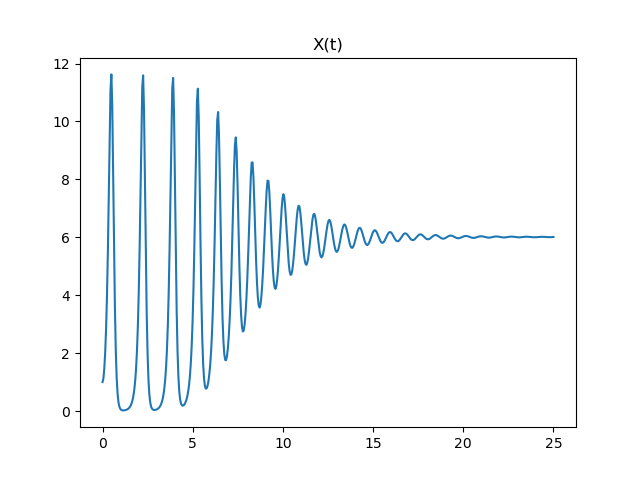
\includegraphics[scale=0.45]{imagenes/punto1/eje_x14.5500.png}}
    \subfigure{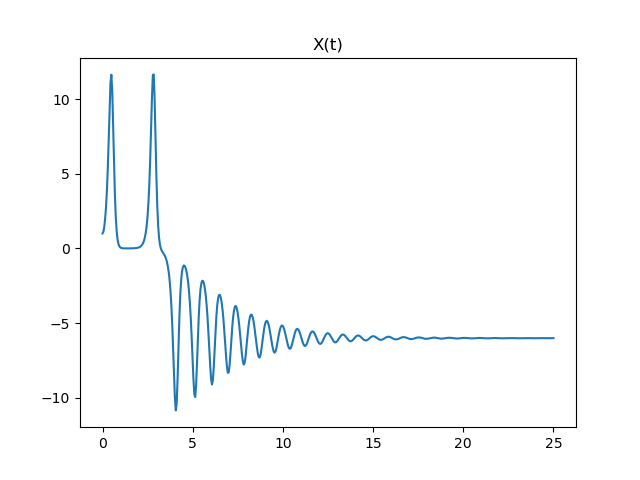
\includegraphics[scale=0.45]{imagenes/punto1/eje_x14.5599.png}}
    \subfigure{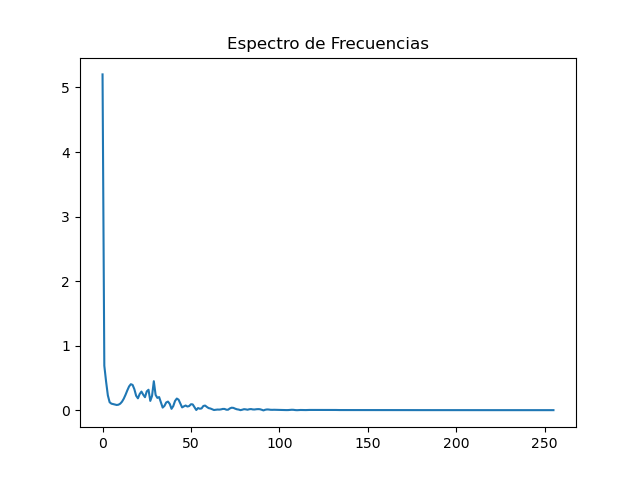
\includegraphics[scale=0.45]{imagenes/punto1/espectro14.5500.png}}
    \subfigure{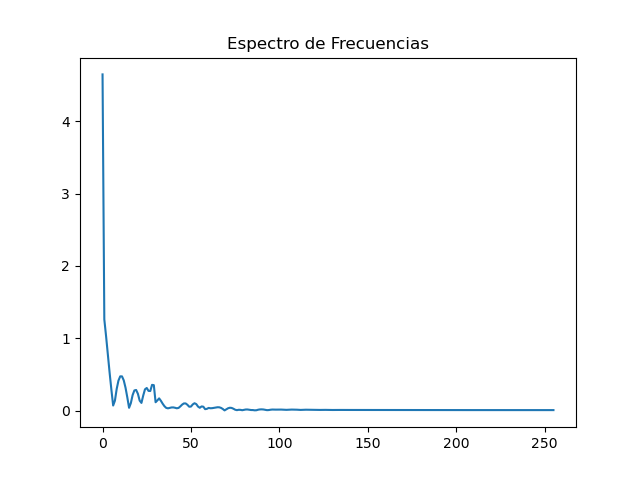
\includegraphics[scale=0.45]{imagenes/punto1/espectro14.5599.png}}
    \subfigure{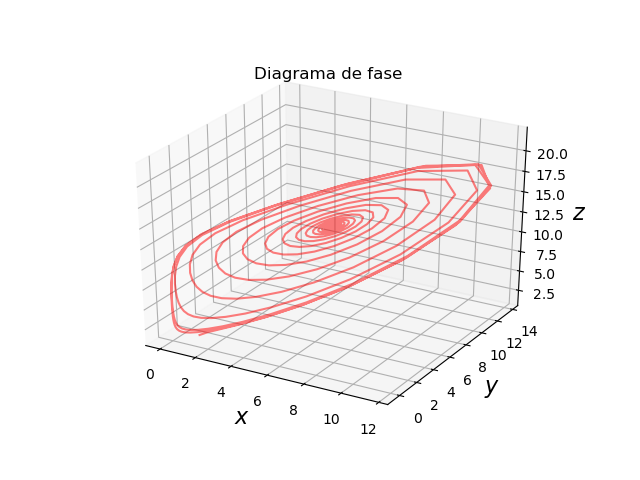
\includegraphics[scale=0.45]{imagenes/punto1/fase14.5500.png}}
    \subfigure{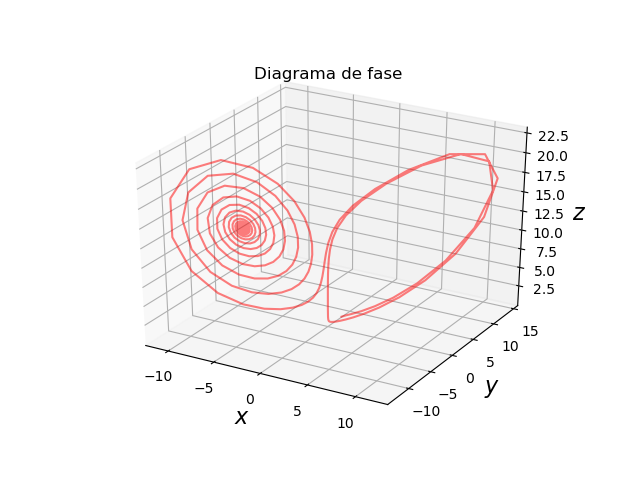
\includegraphics[scale=0.45]{imagenes/punto1/fase14.5599.png}}
    \caption{\emph{$\rho = 14.5500 \Longrightarrow \rho = 14.5899 $}}
\end{figure}

\begin{figure}[H]
    \centering
    \subfigure{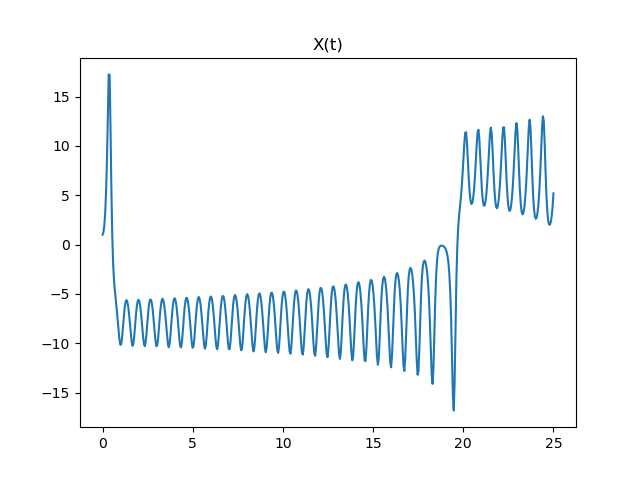
\includegraphics[scale=0.45]{imagenes/punto2/eje_x97.png}}
    \subfigure{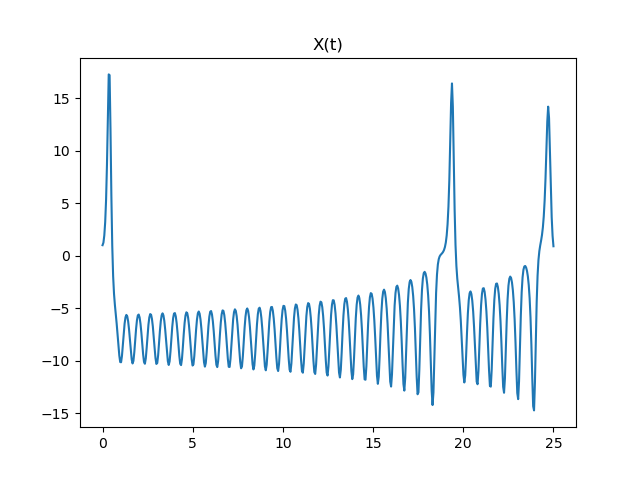
\includegraphics[scale=0.45]{imagenes/punto2/eje_x98.png}}
    \subfigure{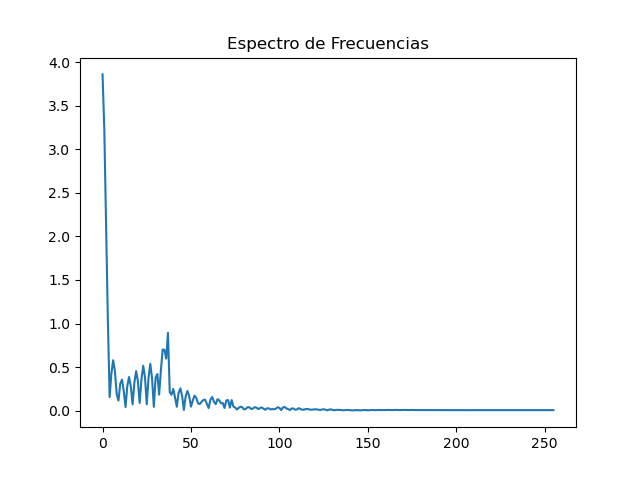
\includegraphics[scale=0.45]{imagenes/punto2/espectro97.png}}
    \subfigure{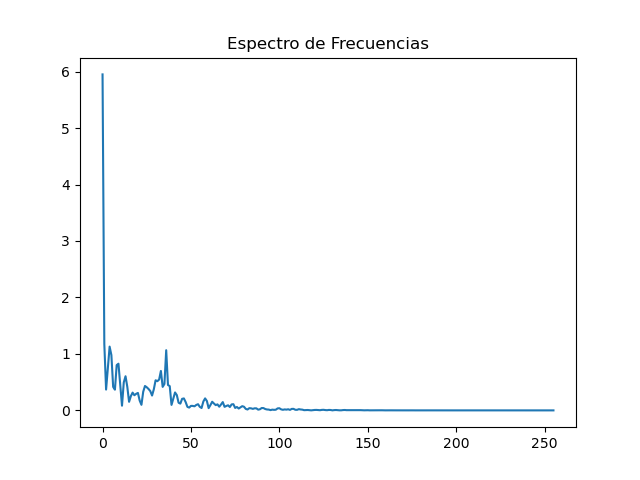
\includegraphics[scale=0.45]{imagenes/punto2/espectro98.png}}
    \subfigure{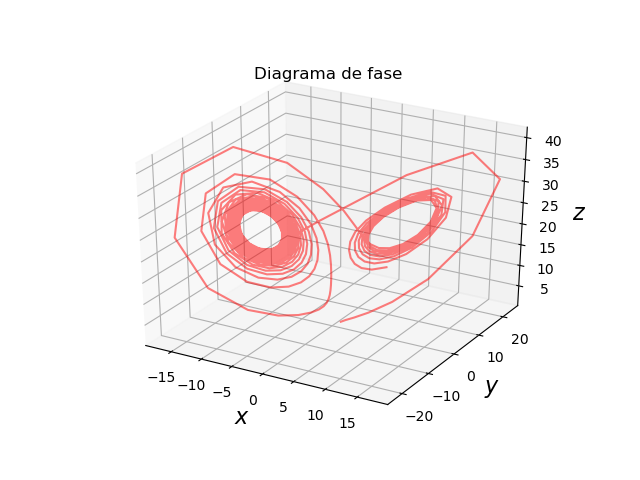
\includegraphics[scale=0.45]{imagenes/punto2/fase97.png}}
    \subfigure{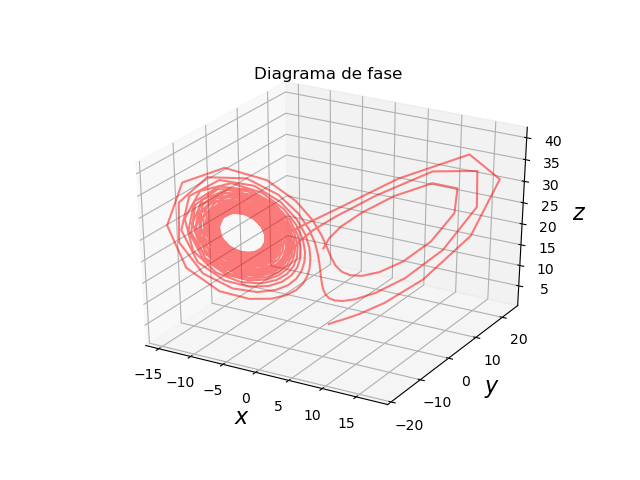
\includegraphics[scale=0.45]{imagenes/punto2/fase98.png}}
    \caption{\emph{$\rho = 24.97 \Longrightarrow \rho = 24.98 $}}
\end{figure}

\begin{figure}[H]
    \centering
    \subfigure{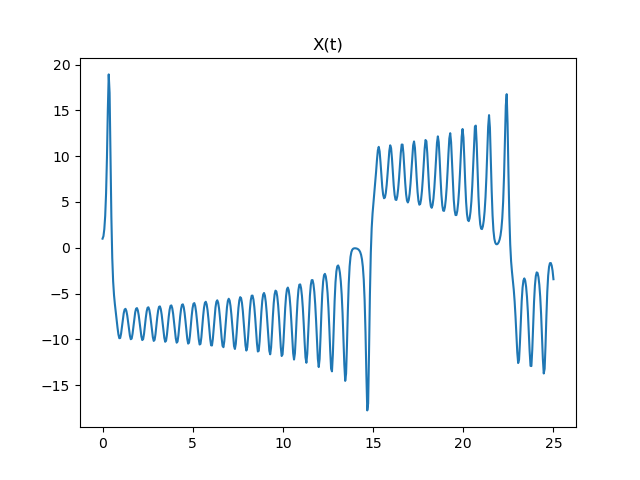
\includegraphics[scale=0.45]{imagenes/punto3/eje_x8.png}}
    \subfigure{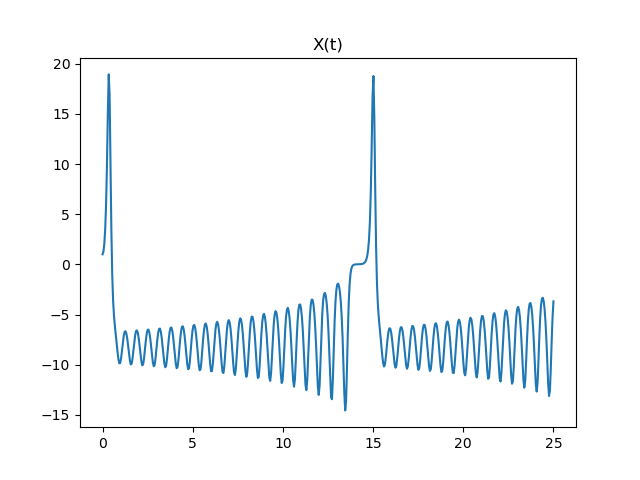
\includegraphics[scale=0.45]{imagenes/punto3/eje_x9.png}}
    \subfigure{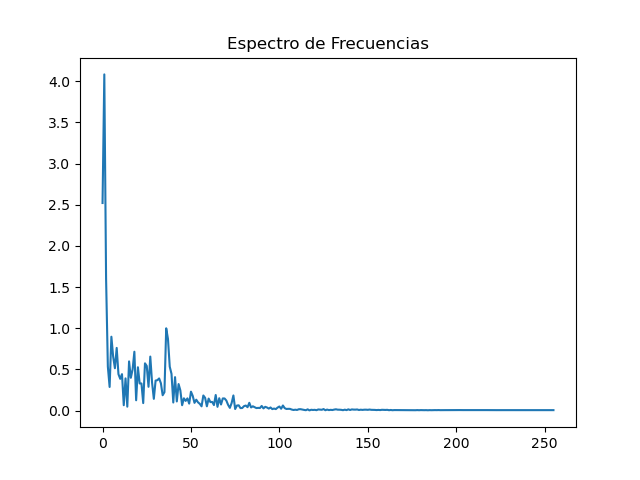
\includegraphics[scale=0.45]{imagenes/punto3/espectro8.png}}
    \subfigure{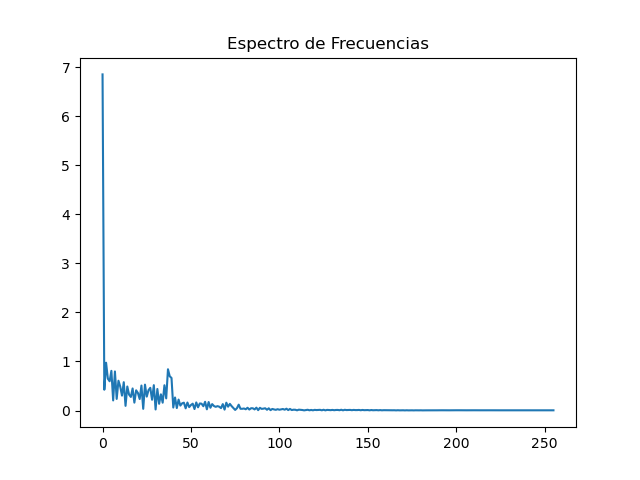
\includegraphics[scale=0.45]{imagenes/punto3/espectro9.png}}
    \subfigure{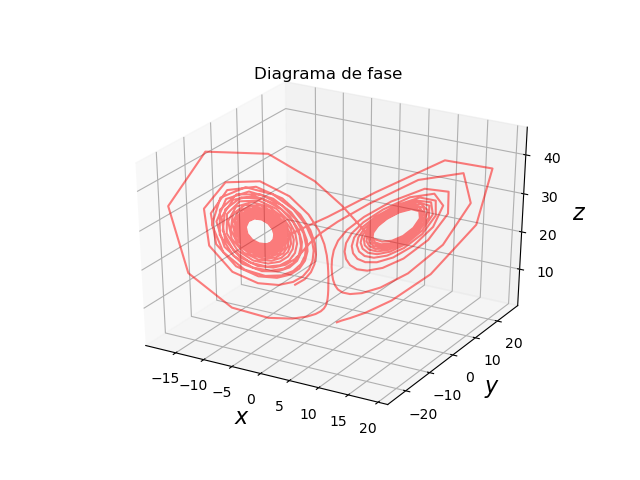
\includegraphics[scale=0.45]{imagenes/punto3/fase8.png}}
    \subfigure{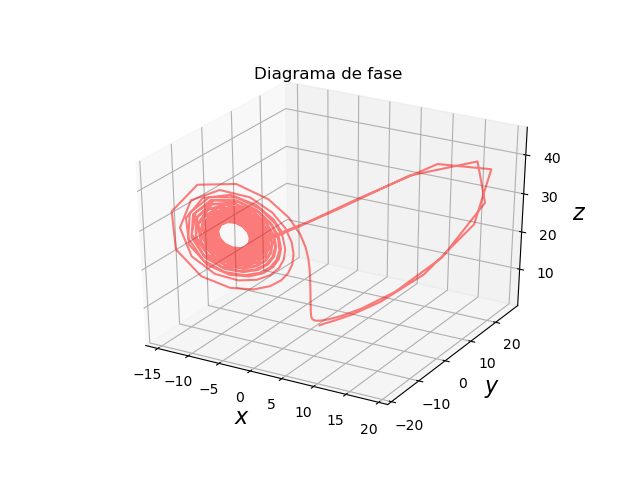
\includegraphics[scale=0.45]{imagenes/punto3/fase9.png}}
    \caption{\emph{$\rho = 27.08 \Longrightarrow \rho = 27.09 $}}
\end{figure}

\twocolumn
